% This is "sig-alternate.tex" V2.0 May 2012
% This file should be compiled with V2.5 of "sig-alternate.cls" May 2012
%
% This example file demonstrates the use of the 'sig-alternate.cls'
% V2.5 LaTeX2e document class file. It is for those submitting
% articles to ACM Conference Proceedings WHO DO NOT WISH TO
% STRICTLY ADHERE TO THE SIGS (PUBS-BOARD-ENDORSED) STYLE.
% The 'sig-alternate.cls' file will produce a similar-looking,
% albeit, 'tighter' paper resulting in, invariably, fewer pages.
%
% ----------------------------------------------------------------------------------------------------------------
% This .tex file (and associated .cls V2.5) produces:
%       1) The Permission Statement
%       2) The Conference (location) Info information
%       3) The Copyright Line with ACM data
%       4) NO page numbers
%
% as against the acm_proc_article-sp.cls file which
% DOES NOT produce 1) thru' 3) above.
%
% Using 'sig-alternate.cls' you have control, however, from within
% the source .tex file, over both the CopyrightYear
% (defaulted to 200X) and the ACM Copyright Data
% (defaulted to X-XXXXX-XX-X/XX/XX).
% e.g.
% \CopyrightYear{2007} will cause 2007 to appear in the copyright line.
% \crdata{0-12345-67-8/90/12} will cause 0-12345-67-8/90/12 to appear in the copyright line.
%
% ---------------------------------------------------------------------------------------------------------------
% This .tex source is an example which *does* use
% the .bib file (from which the .bbl file % is produced).
% REMEMBER HOWEVER: After having produced the .bbl file,
% and prior to final submission, you *NEED* to 'insert'
% your .bbl file into your source .tex file so as to provide
% ONE 'self-contained' source file.
%
% ================= IF YOU HAVE QUESTIONS =======================
% Questions regarding the SIGS styles, SIGS policies and
% procedures, Conferences etc. should be sent to
% Adrienne Griscti (griscti@acm.org)
%
% Technical questions _only_ to
% Gerald Murray (murray@hq.acm.org)
% ===============================================================
%
% For tracking purposes - this is V2.0 - May 2012

\documentclass{sig-alternate}

\usepackage[table]{xcolor}
\usepackage{afterpage}

\begin{document}
%
% --- Author Metadata here ---
% \conferenceinfo{WOODSTOCK}{'97 El Paso, Texas USA}
% \CopyrightYear{2007} % Allows default copyright year (20XX) to be over-ridden - IF NEED BE.
% \crdata{0-12345-67-8/90/01}  % Allows default copyright data (0-89791-88-6/97/05) to be over-ridden - IF NEED BE.
% --- End of Author Metadata ---

\title{On Building An Interpolation System Using Decision Trees}

%
% You need the command \numberofauthors to handle the 'placement
% and alignment' of the authors beneath the title.
%
% For aesthetic reasons, we recommend 'three authors at a time'
% i.e. three 'name/affiliation blocks' be placed beneath the title.
%
% NOTE: You are NOT restricted in how many 'rows' of
% "name/affiliations" may appear. We just ask that you restrict
% the number of 'columns' to three.
%
% Because of the available 'opening page real-estate'
% we ask you to refrain from putting more than six authors
% (two rows with three columns) beneath the article title.
% More than six makes the first-page appear very cluttered indeed.
%
% Use the \alignauthor commands to handle the names
% and affiliations for an 'aesthetic maximum' of six authors.
% Add names, affiliations, addresses for
% the seventh etc. author(s) as the argument for the
% \additionalauthors command.
% These 'additional authors' will be output/set for you
% without further effort on your part as the last section in
% the body of your article BEFORE References or any Appendices.

\numberofauthors{3} %  in this sample file, there are a *total*
% of EIGHT authors. SIX appear on the 'first-page' (for formatting
% reasons) and the remaining two appear in the \additionalauthors section.
%
\author{
% You can go ahead and credit any number of authors here,
% e.g. one 'row of three' or two rows (consisting of one row of three
% and a second row of one, two or three).
%
% The command \alignauthor (no curly braces needed) should
% precede each author name, affiliation/snail-mail address and
% e-mail address. Additionally, tag each line of
% affiliation/address with \affaddr, and tag the
% e-mail address with \email.
%
\alignauthor
    Amy Briggs \\
   \email{abbr5@mst.edu}
\alignauthor
    Andrew Fallgren \\
    \email{ajffk6@mst.edu}
\alignauthor
    George Rush \\
    \email{gdr34b@mst.edu}
}

\maketitle
\begin{abstract}
One class of data is measured or simulated data with error estimation. This data can consist of many continuous dimensions for which values are available only at discrete points. Increasing the number of discrete points at which the data is available can be expensive or even impossible to obtain, but it can still be useful for predicting data trends. Unfortunately, this is difficult when the various dimensions do not follow the same type of fit (linear, logarithmic, polynomial, etc.). Our approach focuses on building decision trees and using them to interpolate new data points that follow existing trends. This is in contrast to previous methods which focused on extrapolating data for specific applications or using purely numerical regression models. By using this approach, sparse data sets or those that exhibit unusual patterns can be analyzed effectively.
\end{abstract}

\category{H.2.8}{Database Management}{Database Applications}[data mining]

\terms{Algorithms}

\keywords{data mining, sparse data, interpolation}

\section{Introduction}
There are times when the only class of data available for analysis is measured or simulated data. Collecting such data can be time and labor intensive, and the data points may be sparse at best. As such, it can be worthwhile to use techniques that increase the utility of data points which have already been collected. Interpolation in particular can help to clarify trends within the data by generating new points according to the patterns established by existing data. 

Prior methods of interpolation all work by utilizing different mathematical functions to fit patterns of values. This process can be ineffective if different dimensions or classifications of the data do not fit to a single formula, such as linear, logarithmic, polynomial, et cetera, as then certain formulas would only perform accurately for specific segments of the data.

Our proposed solution first requires modelling the data using decision trees. By doing this, it is possible to group data points by their classification and similar characteristics at various leaf nodes. We then interpolate new data instances based upon the distribution of instances within each of the leaf nodes. This produces interpolated data with a similar distribution and attribute values when compared to the original data set. Also, the new instances retain roughly the same proportion as the original data regarding the number of instances per leaf node.

By using this method against multiple well known test data sets, we demonstrate a proof of concept for its applicability across multiple problem domains.

\section{Related Work}
Early works on the interpolation of scattered data evaluate a variety of different computational methods that focus on obtaining a smooth function $F(x, y)$ to follow the data set. They utilize numerous different mathematical methods including the following: inverse distance weighted method, rectangle based blending method, triangle based blending method, finite element based method, Foley's method, global basis function type method, and modified Maude method \cite{franke1982scattered}. All of these techniques focus only on developing a function in order to interpolate scattered data sets.

Later works build off of that approach, by taking classical radial basis functions, such as Duchon's thin plate splines and Hardy's multiquadratics, and compressing them in order to shorten the excessive computation times that result from applying these functions to large data sets, while trying to maintain a smooth data fitting \cite{floater1996multistep}.

There are reapplications of some of these interpolation functions to generate continuous surfaces from irregularly distributed data, in attempts to analyze which function best for spatial analysis. The methods include: inverse square distance method, Kriging method, tension finite difference method, and Hardy's multiquadric method \cite{caruso1998interpolation}. 

Several cases can be found in which these interpolation functions are modified to more accurately apply to specific data sets. One example is the use of a combination of the thin plate smoothing spline and Kringing method in spatial interpolation in order to create a more comprehensive archive of Australian climate data \cite{jeffrey2001using}. Another uses spatial interpolation in improving the MODIS global data sets for terrestrial gross and net primary production \cite{zhao2005improvements}.

Although more applications of function-based interpolation can be found, we could not locate any use of data mining classification models for interpolation purposes.

\section{Methodology}
\subsection{Decision Tree Interpolation}
Decision Tree Interpolation follows this process:
\begin{enumerate}
    \item Build a decision tree from the original data.
    \item For each leaf node in the tree:
    \begin{enumerate}
        \item Obtain all attribute values for associated data instances.
        \item Define ranges for attribute values.
        \begin{itemize}
            \item For numeric attributes, define the range using minimum and maximum values.
            \item For discrete attributes, define the range as all distinct values.
        \end{itemize}
        \item Calculate the distribution of all associated data instances.
        \item Create new data points within the ranges that match the statistical distribution.
    \end{enumerate}
\end{enumerate}
Note that the number of data points created per leaf node is proportional to the number of data points already classified by that leaf node. This ensures that any interpolated data will follow the overall data distribution, at least relative to the data density per leaf node. 
\begin{table*}[!t]
    \caption{Experiment Result Summary}
    \label{table:experiment_result_summary}
    \centering
    \rowcolors{2}{gray!25}{white}
    \begin{tabular}{cccccc}
        \rowcolor{gray!50}
        \textbf{Data Set} & \textbf{Max Tree Depth} & \textbf{OT -> OD} & \textbf{OT -> ND} & \textbf{NT -> OD} & \textbf{NT -> ND} \\
        adult\_sample & 1 & 0.805527123849 & 0.780737704918 & 0.804503582395 & 0.782786885246 \\
        adult\_sample & 2 & 0.808597748209 & 0.809426229508 & 0.249744114637 & 0.813524590164 \\
        adult\_sample & 3 & 0.816786079836 & 0.850102669405 & 0.801432958035 & 0.852156057495 \\
        adult\_sample & 4 & 0.822927328557 & 0.794661190965 & 0.787103377687 & 0.784394250513 \\
        adult\_sample & 5 & 0.822927328557 & 0.84052532833 & 0.792221084954 & 0.84052532833 \\
        car & 1 & 0.700231481481 & 0.710648148148 & 0.700231481481 & 0.710648148148 \\
        car & 2 & 0.777777777778 & 0.783564814815 & 0.774305555556 & 0.789351851852 \\
        car & 3 & 0.824074074074 & 0.809027777778 & 0.824074074074 & 0.815972222222 \\
        car & 4 & 0.894097222222 & 0.903935185185 & 0.889467592593 & 0.915509259259 \\
        car & 5 & 0.96412037037 & 0.966981132075 & 0.938078703704 & 0.982311320755 \\
        iris & 1 & 0.666666666667 & 0.693333333333 & 0.666666666667 & 0.693333333333 \\
        iris & 2 & 0.96 & 0.973333333333 & 0.946666666667 & 0.986666666667 \\
        iris & 3 & 0.973333333333 & 0.959459459459 & 0.953333333333 & 0.972972972973 \\
        iris & 4 & 0.98 & 0.959459459459 & 0.946666666667 & 1.0 \\
        iris & 5 & 1.0 & 1.0 & 0.966666666667 & 1.0 \\
        lung-cancer & 1 & 0.59375 & 0.6 & 0.375 & 0.666666666667 \\
        lung-cancer & 2 & 0.625 & 0.571428571429 & 0.4375 & 0.714285714286 \\
        lung-cancer & 3 & 0.625 & 0.642857142857 & 0.5625 & 1.0 \\
        lung-cancer & 4 & 0.6875 & 0.428571428571 & 0.53125 & 1.0 \\
        lung-cancer & 5 & 0.78125 & 0.538461538462 & 0.53125 & 1.0 \\
        tic\_tac\_toe & 1 & 0.699373695198 & 0.68267223382 & 0.699373695198 & 0.68267223382 \\
        tic\_tac\_toe & 2 & 0.705636743215 & 0.690376569038 & 0.703549060543 & 0.696652719665 \\
        tic\_tac\_toe & 3 & 0.769311064718 & 0.779874213836 & 0.755741127349 & 0.758909853249 \\
        tic\_tac\_toe & 4 & 0.831941544885 & 0.82264957265 & 0.745302713987 & 0.856837606838 \\
        tic\_tac\_toe & 5 & 0.918580375783 & 0.907284768212 & 0.83611691023 & 0.933774834437 \\
        voting & 1 & 0.95632183908 & 0.923766816143 & 0.95632183908 & 0.923766816143 \\
        voting & 2 & 0.95632183908 & 0.956896551724 & 0.95632183908 & 0.956896551724 \\
        voting & 3 & 0.963218390805 & 0.913357400722 & 0.95632183908 & 0.927797833935 \\
        voting & 4 & 0.963218390805 & 0.892156862745 & 0.928735632184 & 0.90522875817 \\
        voting & 5 & 0.972413793103 & 0.866071428571 & 0.937931034483 & 0.895833333333 \\
    \end{tabular}
\end{table*}

\subsection{Interpolated Data Validation}
All interpolated data is validated through this process:
\begin{enumerate}
    \item A new decision tree is built based on the interpolated data. Note that the original data is \textit{not} included here.
    \item Both the new and original decision trees are compared for accuracy against the new and original data sets.
\end{enumerate}
Note that any decision tree with an arbitrarily large maximum depth can classify data with perfect accuracy. Defining a low maximum depth means that classification is imperfect, and it is under these conditions that differences in the quality of different decision trees become apparent.

\subsection{Experiment Parameters}
We completed 30 experiments based on two variables: data source and maximum depth of the decision tree. The maximum depth ranged from one to five, and there were six data sources pulled from Orange's documentation data sets.

\section{Results}
Result data is shown in Table~\ref{table:experiment_result_summary}. The first two columns list the data source and the maximum depth for generated decision trees. Note that two decision trees are generated per row, one for the original data and one for the new (interpolated) data. The last four columns list the accuracy of both the original and new decision trees against the original and new data sets. For example, the column labeled "OT -> ND" shows the accuracy of the original decision tree (OT) when used to classify instances in the new data set (ND). Results and outliers for each of the data sets will be explored further here.
\subsection{adult\_sample}
The only significant outlier in this group was for a max tree depth of two. The "NT -> OD" column shows an accuracy of 0.2497 while the other accuracy values ranged from 0.8085 to 0.8135. Ignoring the outlier, accuracy ranged from 0.7807 to 0.8522 for this data source.
\subsection{car}
Results in this section largely followed expected trends. Accuracy ranged from 0.7002 to 0.9823 for this data source, and accuracy increased in each column as the max tree depth increased.
\subsection{iris}
Results in this section followed expectations, but classification started out relatively inaccurate. At a max tree depth of 1, accuracy ranged from 0.6667 to 0.6933. At a max tree depth of 2, accuracy increased rapidly to range from 0.9467 to 0.9867. Accuracy remained above 0.9467 for all other entries.
\subsection{lung-cancer}
Accuracy had enormous variance here, ranging from 0.375 to 1.0 across all categories. While both decision trees increased in accuracy as max depth increased for their own data sets, they did not consistently increase in accuracy for the other data set.
\subsection{tic\_tac\_toe}
Results in this section were mostly consistent, and accuracy ranged from 0.6827 to 0.9338. Accuracy tended to increase as max tree depth increased, with only slight exceptions.
\subsection{voting}
While there was no clear trend in the results for this data source, accuracy was consistently greater than or equal to 0.8661 for all entries. All but three values were above 0.9, so accuracy was generally high across all instances.

\section{Discussion}
In general, points generated by our algorithm were classified with similar accuracy to the original data. In cases where the tree generated from the original data classified that data poorly, the newly generated data had the same behavior. In cases where the original data was classified with high reliability, the same was true for the interpolated points. This is a positive outcome as the goal is to generate new instances of data that behave similarly to the old instances, as opposed to generating instances which would be predicted with any particular accuracy by the decision tree.

There are two main cases for which the generated data does not produce a tree which provides similar classification to the original tree: the adult\_sample data set with a maximum depth of two and the lung-cancer data set in general.

In the original set of experiments, 0.5 data points were generated for each original data point assigned to a leaf. In exploring possible reasons for the discrepancies in how closely the generated data matched the original, this parameter was increased. As it was increased, the old data was classified by the new decision tree with similar accuracy to that of the new data and to the accuracy of the original tree. This suggests that false trends were being created by statistical noise when not enough new points were generated. In the case of the adult\_sample data set with depth two, it is purely an artifact of using random selection and a particular combination of random seed and data. For the lung cancer data, this type of statistical noise can be expected to be a larger problem as the data set has a large number of fields, but only a few possible values for each of those fields.

\section{Conclusion and Future Work}
This initial investigation showed that it is possible to use our method to generate new data points that behave similarly to the original data regarding their classification. As the selection of values is done in a relatively simple way, a large number of new data points can be generated quickly. This generated data can then be used as a substitute for the original data without many of the privacy concerns or other issues that might restrict the use of such data. This approach worked on multiple types of data, both continuous and discrete values, and on varying sized data sets.

Future work in this area would be to more fully explore the optimum selection of parameters used in the algorithm. In the case of this paper, continuous data was binned into 20 discrete bins, and values were chosen from within a bin with equal probability. This level of discretization worked for the data sets examined, but there is no reason to expect this would always be the case. Another parameter that was shown to have impact is the number of new data points to generate. A larger set of generated points seems to produce better solutions, but this correlation has not been adequately explored to make definitive statements.

For any decision node in our algorithm, there is also no consideration of the possible correlation between fields. We implicitly assume that said correlation is unnecessary for our method of interpolation. This assumption works well if the original decision tree has already captured these correlations in resulting model, but in the cases where that is not true, expansion of the algorithm to include correlation between fields may increase the usefulness of the generated points. 

%\end{document}  % This is where a 'short' article might terminate

%
% The following two commands are all you need in the
% initial runs of your .tex file to
% produce the bibliography for the citations in your paper.
\bibliographystyle{abbrv}
\bibliography{references}  % references.bib is the name of the Bibliography in this case
% You must have a proper ".bib" file
%  and remember to run:
% latex bibtex latex latex
% to resolve all references
%
% ACM needs 'a single self-contained file'!

\appendix
\section{Example Decision Trees}
In the following pages, we display some of the decision trees from our experiments. Each tree is labeled with the corresponding data set name, whether it was generated from the original or interpolated data, and the maximum depth. For each data set, we chose to display decision trees at the highest maximum depth that was viewable in this format. This is because some decision trees at depth five were impossible to examine when resized to fit on one page. This section is meant to demonstrate how the complexity of decision trees can vary depending on the data set, but it also provides a visual contrast of the decision tree structure for original versus interpolated data.

\clearpage
\begin{figure*}[!t]
    \centering
    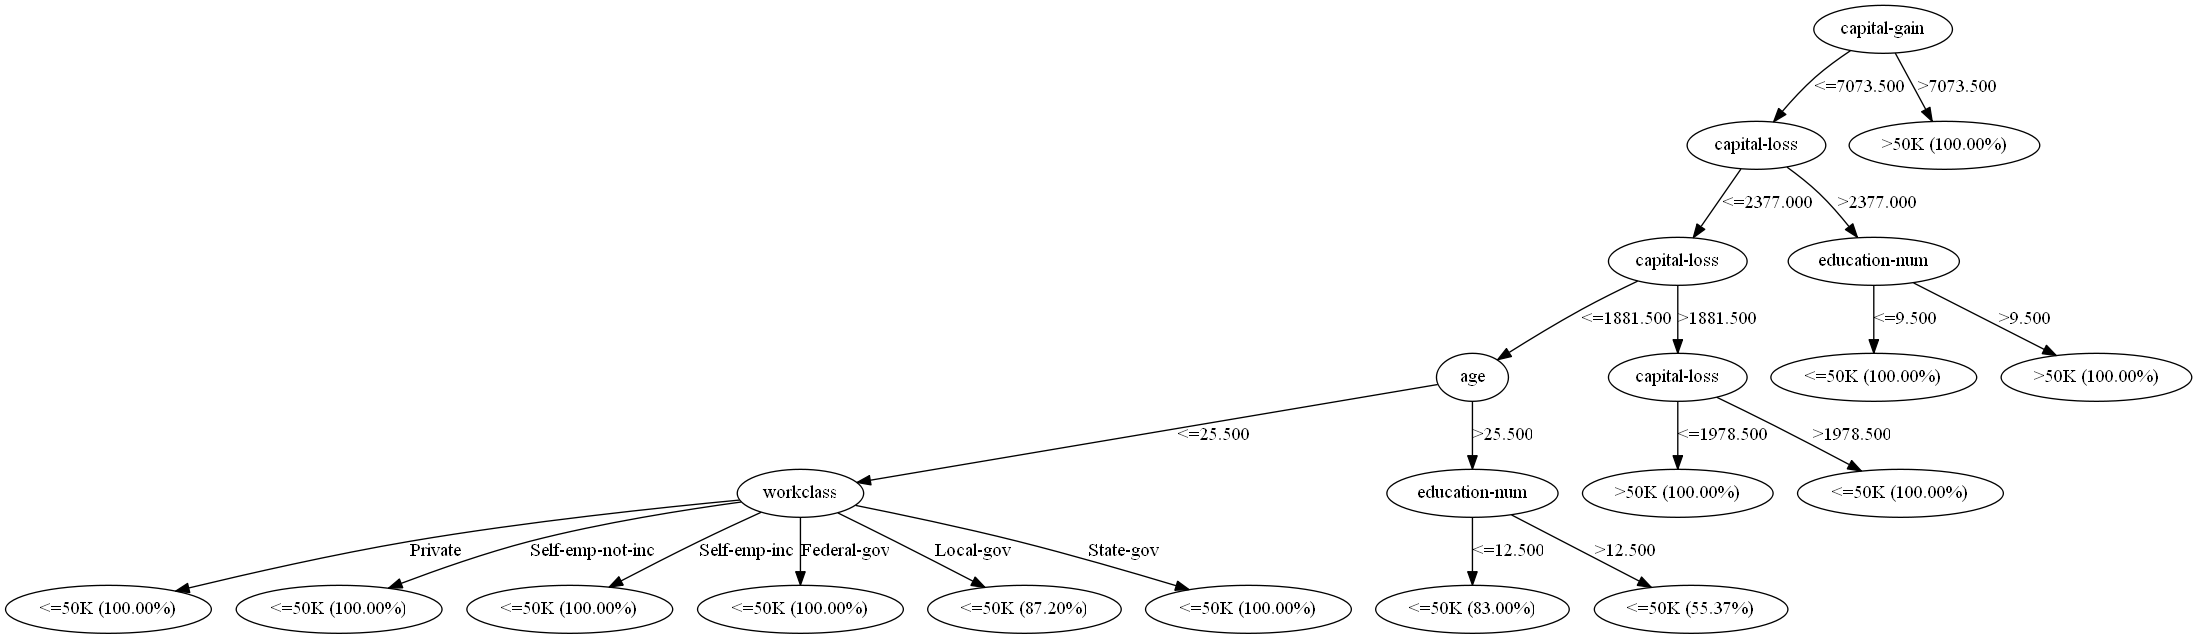
\includegraphics[width=1.00\textwidth,height=10cm,keepaspectratio]{./images/adultSampleD5Original.png}
    \caption{adult\_sample - original - max depth 5}
    \label{figure:adultSampleD5Original}
\end{figure*}
\begin{figure*}[h]
    \centering
    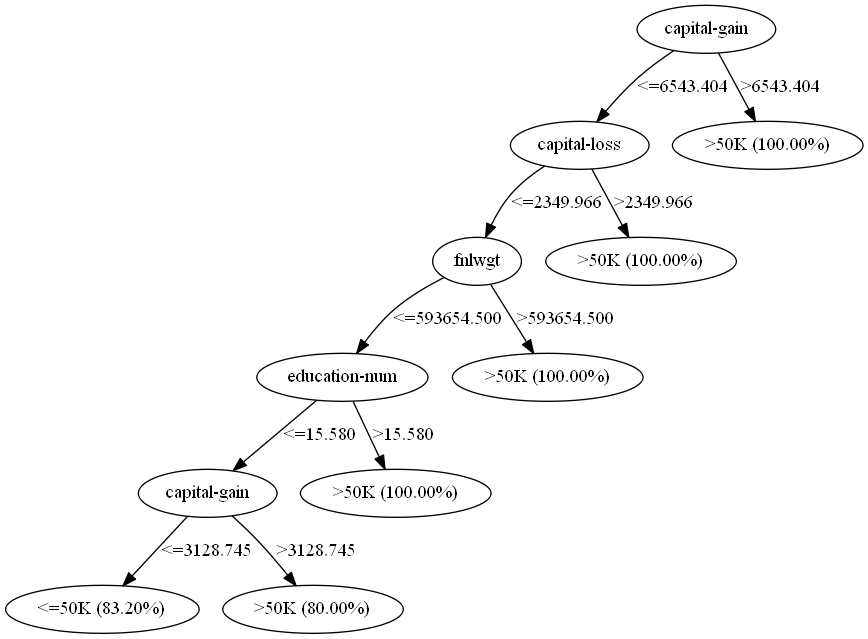
\includegraphics[width=1.00\textwidth,height=10cm,keepaspectratio]{./images/adultSampleD5New.png}
    \caption{adult\_sample - interpolated - max depth 5}
    \label{figure:adultSampleD5New}
\end{figure*}

\clearpage
\begin{figure*}[!t]
    \centering
    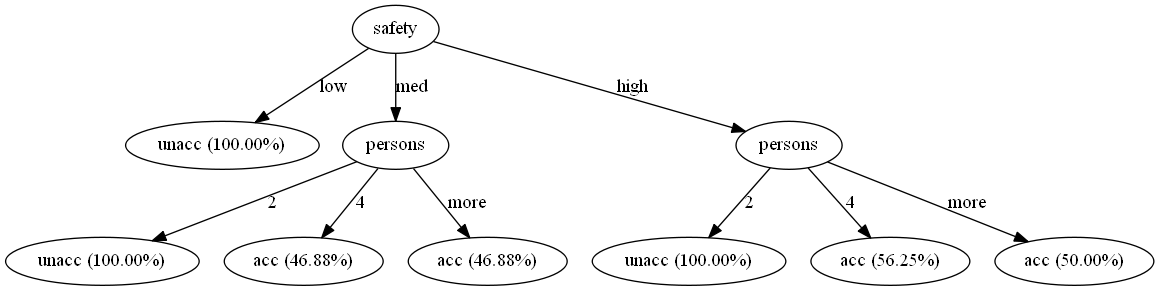
\includegraphics[width=1.00\textwidth,height=10cm,keepaspectratio]{./images/carD2Original.png}
    \caption{car - original - max depth 2}
    \label{figure:carD2Original}
\end{figure*}
\begin{figure*}[h]
    \centering
    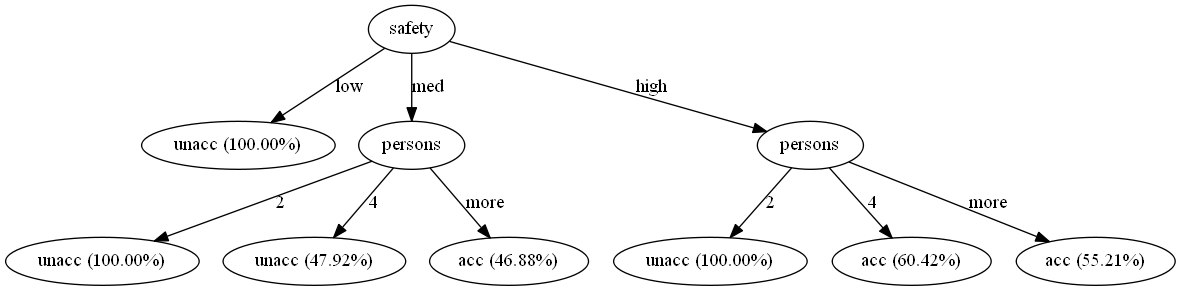
\includegraphics[width=1.00\textwidth,height=10cm,keepaspectratio]{./images/carD2New.png}
    \caption{car - interpolated - max depth 2}
    \label{figure:carD2New}
\end{figure*}

\clearpage
\begin{figure*}[!t]
    \centering
    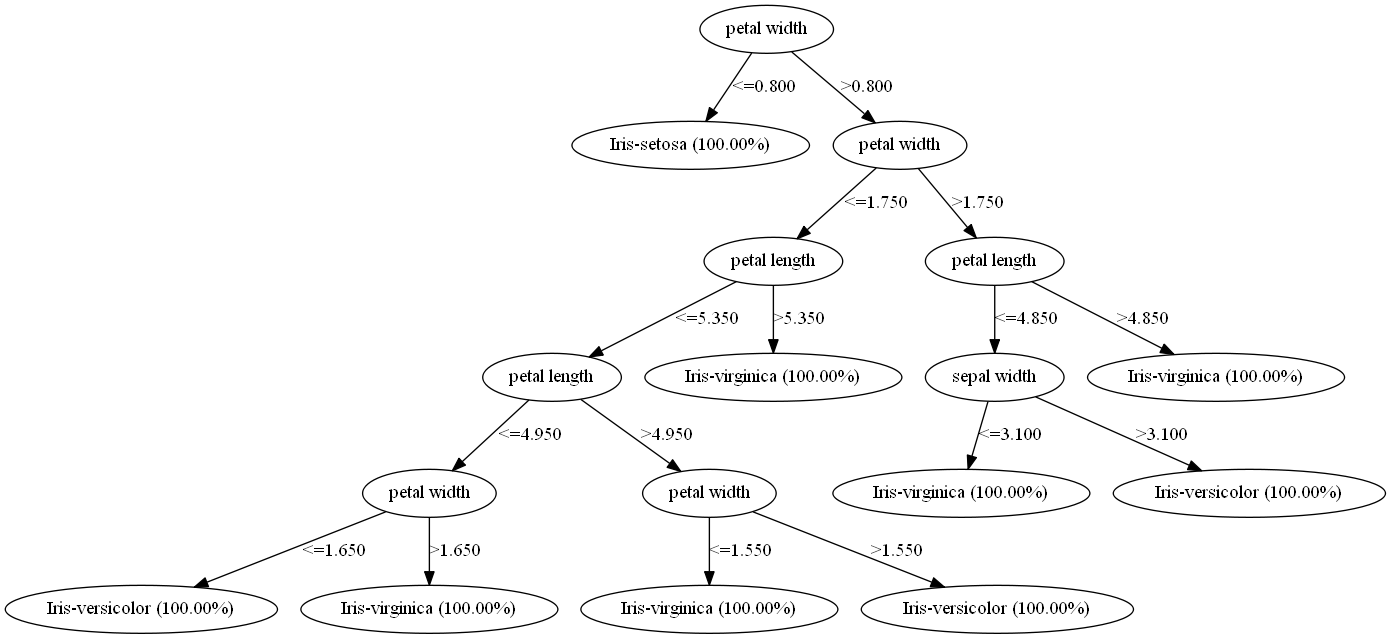
\includegraphics[width=1.00\textwidth,height=10cm,keepaspectratio]{./images/irisD5Original.png}
    \caption{iris - original - max depth 5}
    \label{figure:irisD5Original}
\end{figure*}
\begin{figure*}[h]
    \centering
    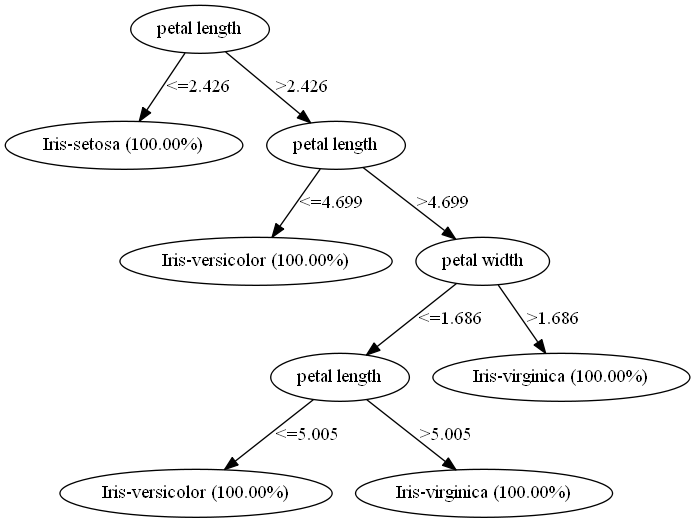
\includegraphics[width=1.00\textwidth,height=10cm,keepaspectratio]{./images/irisD5New.png}
    \caption{iris - interpolated - max depth 5}
    \label{figure:irisD5New}
\end{figure*}

\clearpage
\begin{figure*}[!t]
    \centering
    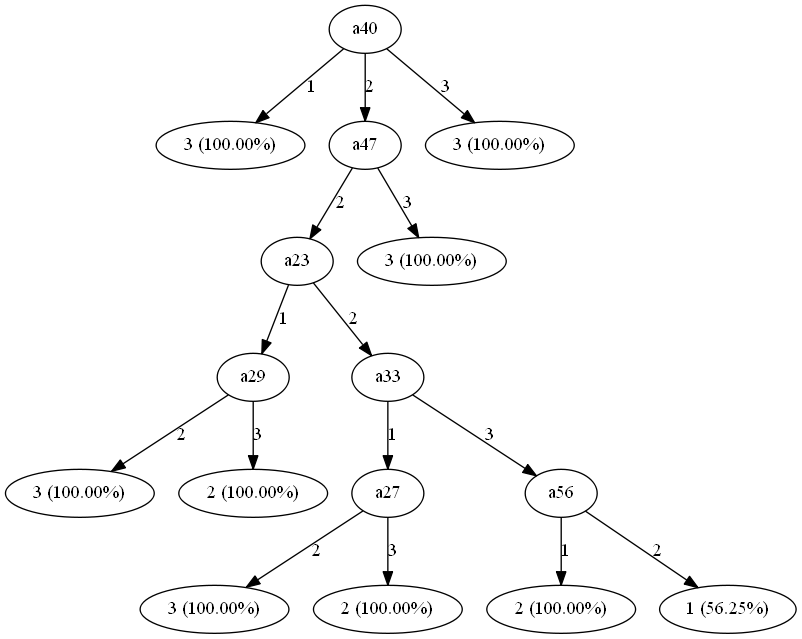
\includegraphics[width=1.00\textwidth,height=10cm,keepaspectratio]{./images/lungCancerD5Original.png}
    \caption{lung-cancer - original - max depth 5}
    \label{figure:lungCancerD5Original}
\end{figure*}
\begin{figure*}[h]
    \centering
    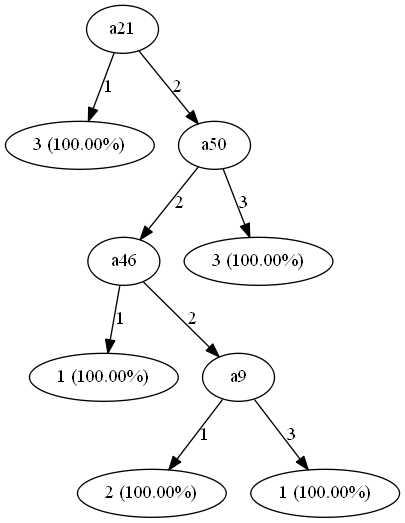
\includegraphics[width=1.00\textwidth,height=10cm,keepaspectratio]{./images/lungCancerD5New.png}
    \caption{lung-cancer - interpolated - max depth 5}
    \label{figure:lungCancerD5New}
\end{figure*}

\afterpage{\clearpage}
\begin{figure*}[!t]
    \centering
    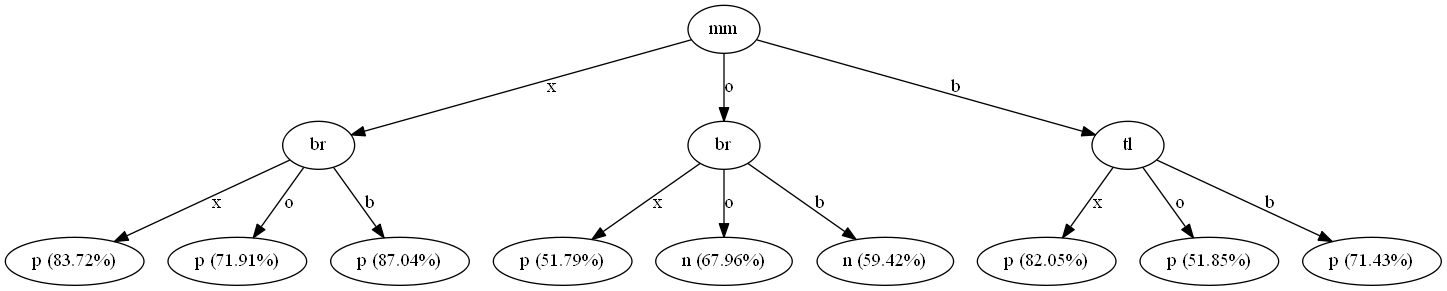
\includegraphics[width=1.00\textwidth,height=10cm,keepaspectratio]{./images/ticTacToeD2Original.png}
    \caption{tic\_tac\_toe - original - max depth 2}
    \label{figure:ticTacToeD2Original}
\end{figure*}
\begin{figure*}[h]
    \centering
    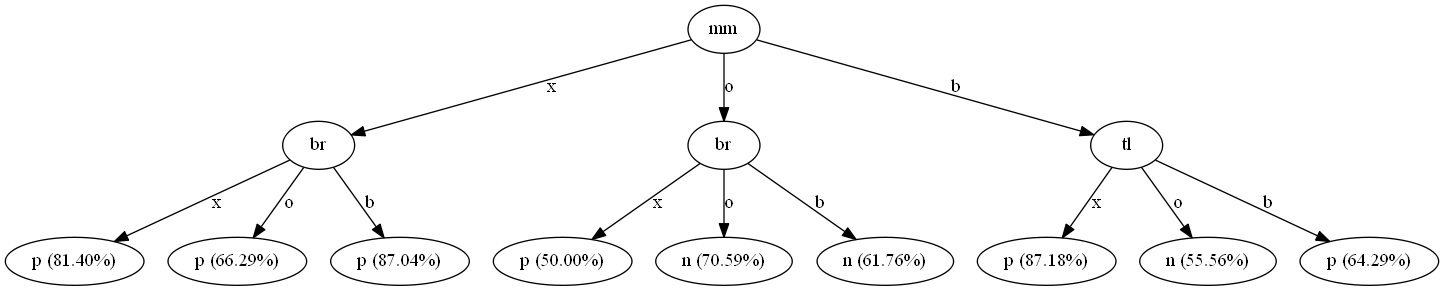
\includegraphics[width=1.00\textwidth,height=10cm,keepaspectratio]{./images/ticTacToeD2New.png}
    \caption{tic\_tac\_toe - interpolated - max depth 2}
    \label{figure:ticTacToeD2New}
\end{figure*}

\clearpage
\begin{figure*}[!t]
    \centering
    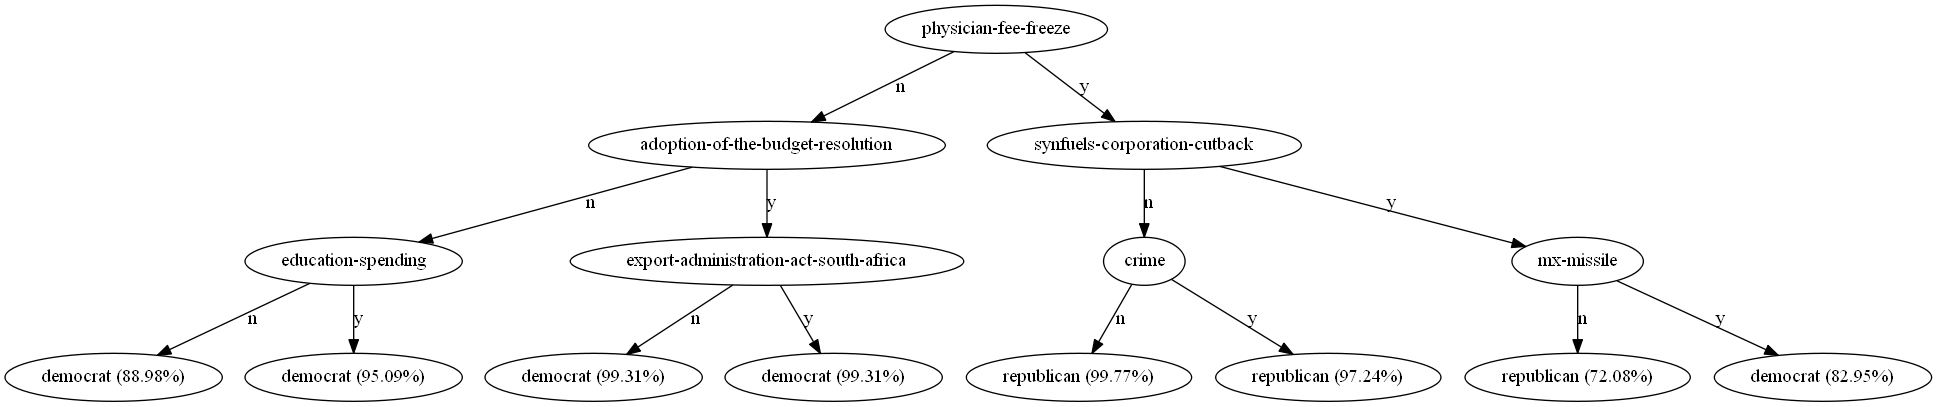
\includegraphics[width=1.00\textwidth,height=10cm,keepaspectratio]{./images/votingD3Original.png}
    \caption{voting - original - max depth 3}
    \label{figure:votingD3Original}
\end{figure*}
\begin{figure*}[h]
    \centering
    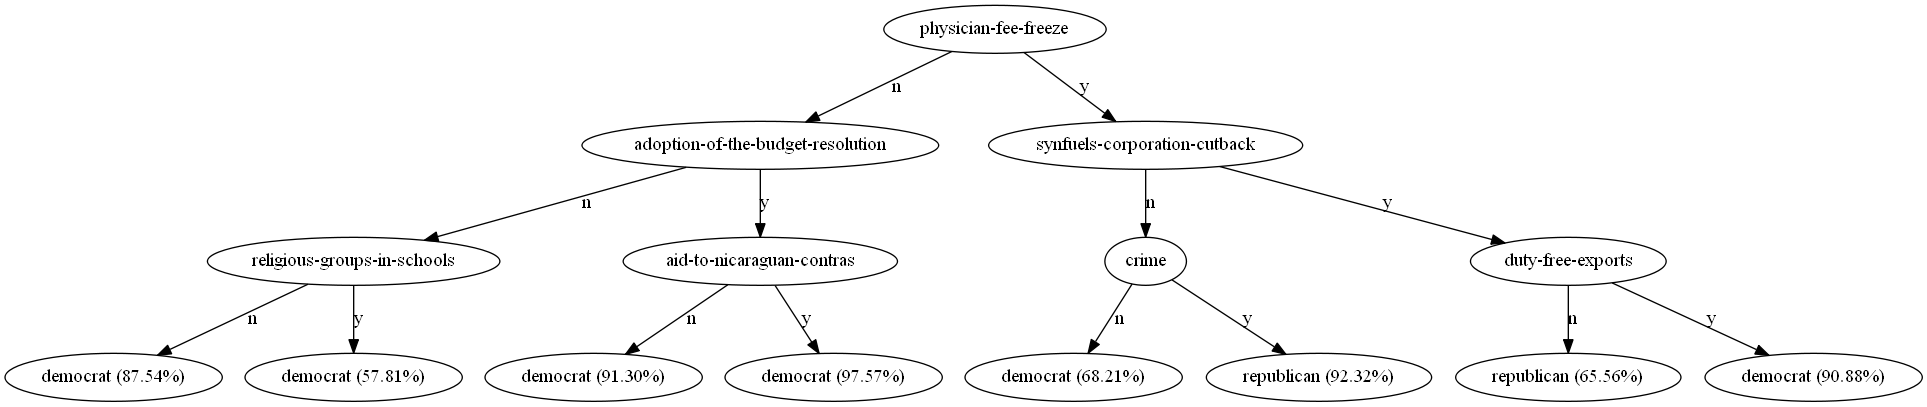
\includegraphics[width=1.00\textwidth,height=10cm,keepaspectratio]{./images/votingD3New.png}
    \caption{voting - interpolated - max depth 3}
    \label{figure:votingD3New}
\end{figure*}

% That's all folks!
\end{document}
